\cotefile{151}

\scanpage{36}
\[
(18)\qquad \varphi:\ p^*(E_{Y,X})\longrightarrow i^*(E_{X^*}).
\]

En termes du diagramme de groupes
$(\unsure{10|1^\circ})$ Quand les \inserted{trois} groupoïdes composants de
(8) sont connexes, i.e. $Y$, $X^*$ et $\mathcal V^*_{Y,X}$
connexes), on peut aussi interpréter
ces systèmes, \deleted{\unsure{comme des systèmes|comme un système}}\inserted{en considérant $E_{X^*}$ comme}
un ens. sur lequel $\Pi_1(X^*)$ opère, $E_{Y,X}$
comme un ens. sur lequel $\Pi_1(Y)$ opère,
et $p^*(E_{Y,X})$ et $i^*(E_{X^*})$ dans (18) comme
étant ces $=$s ensembles, \deleted{\unsure{munis}}\inserted{considérés} comme
$\Pi_1(\mathcal V^*_{Y,X})$-ensembles \deleted{qui} par restriction
des opérateurs.

\margin{NB Dans le cas où on a $=$ un
diagramme (14), cela veut que $\Pi_1(Y)$
apparaît comme un quotient de $D=\Pi_1(\mathcal V^*_{Y,X})$, et
donc $E_{Y,X}$ peut s'interpréter d'emblée comme
un $\deleted{\unsure{\Pi_1(\mathcal V^*_{Y,X})}}D$-ens., sur lequel le \unsure{ss-gr.}
$I$ opère trivialement, on
interprète $\varphi$ de (18) comme un
hom de $\Pi_1(Y)$-ens.
\[
(18\ \mathrm{bis})\qquad E_{Y,X}\longrightarrow
\underbrace{E^I_{X^*}}_{I\text{-invariants}}
\]}

Un cas \inserted{typique,} particulièrement important
pour \unsure{la|les} \deleted{applic. à} Géométrie algébrique,
est celui où $X$ est une surface
top. et où $Y$ est réduit à un pt $a$,
donc $\mathcal V_{Y,a}=\mathbb D_a$, \uline{disque} \inserted{(infinitésimal)} autour de $a$,
et $\mathcal V^*_{Y,a}=\mathbb D^*_0$, disque épointé (inf.) autour
de $a$, de sorte qu'on trouve le diagramme
% Pale bottom-left foliation, in another hand; not the author's own numbering.
\margin{35}

\scanpage{38}
domaine analytique complexe). Ici
$X=\mathbb C$ est topologiquement trivial, ce qui
peut s'exprimer ainsi par le fait que
son type d'homotopie est complètement
décrit par celui du topos $\unsure{\mathcal F|\mathfrak F}$ des
systèmes (17). En effet, on aura
\[
(22)\qquad \unsure{\mathcal F|\mathfrak F}\simeq\widehat C
\]
où $C$ (dans le cas général \deleted{du}\inserted{où dans le} diagramme
(19) \deleted{\unsure{avec $\pi_1(Y)$ réduit à $\{1\}$}}
\inserted{où $\pi_1(Y)=\{1\}$},
\inserted{$D\Rightarrow\pi_1(\mathcal V^*_{Y,X})\xrightarrow{\sim}\pi_1(X^{\unsure{*|\ell}})$ iso)}
\deleted{\unsure{alors}}) est \unsure{défini|définie} comme la catégorie dont
l'ens des objets est l'ens \deleted{\unsure{somme}}\inserted{$\{a,b\}$,}
\deleted{\unsure{réunion} \illegible{3} \unsure{des trois}}
\deleted{\unsure{flèches de sous-catégorie}}
\deleted{\unsure{des ens d'objets} des groupoïdes, composants
\inserted{\unsure{figurer en la} \deleted{\unsure{une}} catégorie}
de (8), et dont les flèches sont, en plus
des flèches de ces trois groupoïdes, les
flèches $\deleted{\unsure{p}}$ d'un objet $a$ de $\inserted{A=}\Pi_1\mathcal V^*_{Y,X}$
vers un objet soit de $B=\Pi_1\deleted{\unsure{\mathcal V_{Y,X}|\mathcal V^*_{Y,X}}}\inserted{\unsure{Y}}$, soit de
$C=\Pi_1\deleted{\unsure{\mathcal V_{Y,X}|\mathcal V^*_{Y,X}}}\inserted{X^*}$, \unsure{définies|définis} comme étant
les flèches :
\[
\deleted{\unsure{\varphi}}\quad p_*(a)\longrightarrow b\quad\text{dans }B
\quad(\text{resp. }j_*(a)\longrightarrow c\quad\text{dans }C).
\]
Dans le cas \deleted{\unsure{actuel}}, présent, les groupoïdes
$A,B,C$ et les morphismes entre eux}
% Pale lower-left foliation, in another hand; not the author's page number.
\margin{37}

\scanpage{39}
\mspage{7}
où $I=D$ est le groupe des auto. de $a$, et où
les seules autres flèches, à part les $\gamma\in D$ et
l'identité de $b$, est une flèche $a\longrightarrow b$ (de
sorte que $b$ est objet final de $C$). Comme
$C$ admet un objet final, $\unsure{\widehat C|\widehat{\mathbb C}}$ \deleted{\unsure{est|et}} (donc aussi
$\unsure{\mathcal F|\mathfrak F}$) est de type d'homotopie trivial ($\infty$-\unsure{connexe|conn}),
ce qui signifie bien que $\unsure{\mathcal F|\mathfrak F}$ a le type d'
homotopie de $\deleted{\unsure{\mathbb C|C}}X=\mathbb C$.

Prenons maintenant le cas où $X$ est le
compactifié $\mathbb P^1_{\mathbb C}$ de $\mathbb C$ par un pt à l'infini,
\deleted{\unsure{donc}}\inserted{disons}
\[
\left\{\begin{array}{l}
X=\mathbb P^1_{\mathbb C}\simeq S^2\\
Y=\{\infty\}
\end{array}\right.
\]
\[
X^*=\deleted{\unsure{\mathbb P}}\mathbb C
\]
le diagramme (7) devient

\noindent (23)
\diagram{\begin{tikzcd}[row sep=large]
\mathbb D^*_{\infty} \arrow[r,hook,no head] \arrow[d] & \mathbb D_{\infty} \arrow[d,dotted] \\
\mathbb C \arrow[r,dashed] & \mathbb P^1_{\mathbb C}\simeq S^2
\end{tikzcd}}

dont la somme amalgamée est $S^2$, dont
le type d'homotopie n'a rien de trivial !
Le topos $\unsure{\mathcal F|\mathfrak F}$ se décrit maintenant à
l'aide du diagramme correspondant sur \unsure{les|le} $\Pi_1$,
savoir
% Pale foliation at the bottom left, in another hand.
\margin{38}

\scanpage{40}
\noindent (23)
\diagram{\begin{tikzcd}
\mathbb Z\arrow[r]\arrow[d]&1\\
1
\end{tikzcd}},
on a maintenant une équivalence de topos
\[
\deleted{\unsure{(24)|(23)}}\qquad \unsure{\mathcal F|\mathfrak F}\approxeq\widehat C,
\]
où $C$ est la catégorie \diagram{\begin{tikzcd}[column sep=small]\bullet\arrow[r]&\bullet\end{tikzcd}}, qui a
un objet final --- donc $\unsure{\mathcal F|\mathfrak F}$ \uline{est encore}
\uline{homotopiquement trivial,} \uline{alors que cette}
\uline{fois-ci $X$ ne l'est pas} ! Pourtant les
\unsure{pierres|pièces} de construction $\{a\}$, $X^*\simeq\mathbb C$, et
${\unsure{V|\mathcal V|Z}}^*_{z,Z}\simeq\mathbb D^*_{\infty}$ sont bel et bien des $K(\pi,1)$ ---
(les deux premières $\unsure{\overline m|=}$ \unsure{contractile|contractiles|contractibles} !). Cela
montre que le topos $\unsure{\mathcal F|\mathfrak F}$, \deleted{\unsure{$\overline m$ si les|$=$ si les}}\inserted{qui en}
principe semblait ``tenir compte'' des
$\Pi_1$ des \unsure{``}\unsure{pierres|pièces} de construction'' $Y,X^*,\mathcal V^*_{Y,X}$,
ne donne pas \inserted{néanmoins} le type d'homotopie
de $X$, $\unsure{=|\overline m}$ si les \unsure{``}morceaux'' sont des
$K(\pi,1)$ --- en d'autres termes, le
morphisme canonique
\[
(24)\qquad X\longrightarrow\unsure{\mathcal F|\mathfrak F}
\]
n'est pas néc\textsuperscript{t} une équivalence d'homotopie.
% Pale foliation at the lower left, in another hand.
\margin{39}

\scanpage{41}
\mspage{8}
J'avais craint un moment, par cet exemple,
que le type total d'homotopie \inserted{de $X$} ne pourrait
pas (avec les hypothèses \inserted{$K(\pi,1)$} faites) se récupérer
à partir de ceux de $X^*$, $Y$, $\mathcal V^*_{Y,X}$ et du
diagramme (7), i.e du diagramme (8)
ou (10). Mais je me suis convaincu ensuite
que cette crainte n'était pas fondée, $\unsure{\overline m|=}$ si
le topos $\unsure{\mathcal F|\mathfrak F}$ n'est pas suffisant, lui, pour
exprimer le type d'homotopie \unsure{correct|courant}.
Essayons en effet, dans le cas qui nous
occupe --- le cas de la division cellulaire
la plus simple de $S^{\unsure{2|7}}$, (qui est en $\unsure{=|\overline m}$ temps
\deleted{élémentaire}
le cas le plus \deleted{simple} élémentaire d'un
diviseur sur une courbe alg complexe
compacte !) --- de récupérer le $H^2(X,A)$
($A$ un groupe de coeff comm, disons),
à partir du diagramme (23). J'interprète
$H^2(X,A)$ comme classifiant les \uline{gerbes} sur
$X$ liées par $A$ --- et je note que pour des
\deleted{telles} gerbes \inserted{sur des topos}, on a une théorie de ``recolle-
% Pale bottom-left foliation, another hand; distinct from the author's 8.
\margin{40}

\scanpage{42}
ment'' évidente, qui ici dit \deleted{\unsure{qu'}}\inserted{que la donnée}
d'une gerbe \inserted{$\mathcal G_X$}
sur $X$, revient à celle de \unsure{gerbes|gerbe} $\mathcal G_{X^*}$ sur
$X^*$ et $\mathcal G_{Y,X}$ sur $\mathcal V_{Y,X}$, et d'une
\deleted{iso.}\inserted{équiv.} de \deleted{\unsure{recollem.|recolle|recoller}} gerbes
\[
(24)\qquad \mathcal G_{Y,X}\mid\mathcal V^*_{Y,X}\simeq
\mathcal G_{X^*}\mid\mathcal V^*_{Y,X}.
\]
Or sur un $K(\pi,1)$, une $A$-gerbe
s'interprète canoniquement comme une
\uline{extension} de $\pi$ par $A$. Donc la donnée
\margin{\diagram{\begin{tikzcd}[column sep=small,row sep=small]
D\arrow[r]\arrow[d]&\Pi_1(Y)\\
\Pi_1(X^*)&
\end{tikzcd}}}
d'une gerbe sur $X\deleted{{}\unsure{\simeq} S^2}$\unsure{,} revient à celle
d'\deleted{\unsure{une ext}} deux extensions, l'une de
$\Pi_1(Y)$ par $A$, l'autre de $\Pi_1(X^*)$ par $A$
et d'un isom. entre les deux extensions
de $D$ par $A$ qui s'en déduisent\unsure{,}
par image inverse par les hom (10).
(cette description marche dès que les
``\unsure{pierres|pièces|pavés}'' $Y$, $X'$, $\mathcal V^*_{Y,X}$ sont connexes, et
que leur $\Pi_2$ est nul). Dans le cas
% Pale lower-left foliation, another hand; not authorial page numbering.
\margin{41}

\scanpage{43}
\mspage{9}
élémentaire de $S^2$ \inserted{de (23)}, on trouve donc
que la donnée d'une gerbe sur $S^2$ équivaut
à celle d'un \uline{automorphisme} de
l'extension triviale \deleted{\unsure{sur}} de $\mathbb Z$ par $A$,
donc \unsure{à|:} un élément de $\operatorname{Hom}(\unsure{\mathbb Z|Z},A)\simeq A$,
d'où la valeur correcte
\[
(25)\qquad H^2(S^2,\deleted{\unsure{\mathbb Z|Z}}\inserted{A})\simeq A,
\]
magnifique succès ! Sans aller plus
loin dans des vérifications, ceci me
convainc que l'intuition qu'il y
a une théorie des \deleted{\unsure{limites inductives}\unsure{,}}\inserted{$\underset{\longrightarrow}{\mathrm{Lim}}$}
\unsure{des|de} types d'homotopie (\unsure{avec|ou} un
théorème \unsure{à|:} la \uline{van Kampen}, disant
que le type d'homotopie d'une
$\underline{\mathrm{Lim}}$ de Topos (Topos ``recollé'') est
la $\underline{\mathrm{Lim}}$ des types d'homotopie),
est bien correcte. En principe, pour
\margin{42}

\scanpage{44}
des ``espaces stratifiés'' (en un sens qui
va être précisé plus bas) dont les
``\unsure{pierres|pièces}'' sont des $K(\unsure{\pi|\Pi},1)$, \deleted{\unsure{cela devrait}}\inserted{tels}
les espaces modulaires de Teichmüller
et leurs compactifiés, et \unsure{les|leurs} sous-espaces
\inserted{et voisinages tubulaires parmi ceux-ci}
qu'on peut leur associer grâce à leurs
stratifications canoniques, le type
d'homotopie doit pouvoir s'exprimer
en termes d'un système inductif
convenable (le plus souvent à ens. d'in-
dices fini) de groupoïdes fondamentaux
\unsure{desdites|des dites} \unsure{pierres|pièces}.

Il me semble d'ailleurs après-coup,
réflexion faite, que cette théorie ``d'intégration''
des types d'homotopie, que nébuleusement
je voyais comme liée au grand yoga des
relations entre structures homotopiques (relatives
sur un topos disons) et les $n$-groupoïdes,
est en fait relativement triviale, et
justiciable sans doute de techniques $\frac12$-
simpliciales des plus standart. Il me
faudra revenir là dessus par la suite -
% Pale bottom-left foliation in another hand; no authorial page number at the top.
\margin{43}

\scanpage{45}
\mspage{10}
2. \uline{Stratifications globales} : \uline{formalisme} $\frac12$ \uline{simplicial}
(sans tubes).

Pour simplifier, je vais me placer sur un
espace topologique $X$ --- par la suite $X$
deviendra un topos quelconque. Les construc-
tions qui suivent, relatifs \unsure{à|:} une ``stratifica-
tion globale'', seront ``faisceautisés sur $X$
par la suite, de la façon habituelle ---
ce qui amènera \inserted{alors} à imposer des condi-
tions supplémentaires de connexité et
de locale connexité, qui pour le moment
ne sont pas nécessaires. De même, il n'y
a pas lieu pour le moment de s'en-
combrer d'hypothèses de locale trivialité
normale des plongements d'espaces.

Soit $I$ un ensemble ordonné, \deleted{$\unsure{X_i}$}
\[
(1)\qquad (X_i)_{i\in I},\quad X_i\subset X
\]
une famille de \deleted{\unsure{parties}}\inserted{sous-espaces} de $X$. On suppose
\[
(1')\quad\left\{\begin{aligned}
\text{a)}\quad&\text{Les }X_i\text{ fermés, la famille }(X_i)\text{ localement finie.}\\
\text{b)}\quad&i\leq j\ \Longrightarrow\ X_i\subset X_j.
\end{aligned}\right.
\]
Posant
\[
(2)\qquad X_{\Delta_0}=\coprod_{i\in I}X_i
=\{(x,\unsure{i})\in X\times I\mid x\in X_i\}
\]
on a un morphisme canonique
% Pale bottom-left foliation in another hand, distinct from the author's dark 10.
\margin{44}

\scanpage{46}
\[
(3)\qquad X_{\Delta_0}\longrightarrow X
\]
et l'hypothèse a) signifie que ce
morphisme \deleted{\unsure{(que)|(qui)}} est \uline{fini} --- i.e. propre
\inserted{sépar} et à fibres finies. C'est aussi une
im\uline{mersion locale}.

On introduit une partie fermée
\diagram{\begin{tikzcd}[column sep=small,row sep=large]
(4)\quad &X_{\Delta_1}\arrow[d,equal,"\text{déf}"]\arrow[r,phantom,"\subset"]&X_{\Delta_0}\times X_{\Delta_0}=\displaystyle\coprod_{(i,j)\in I\times I}X_i\times X_j\\
&\displaystyle\coprod_{i\leq j}\Gamma_{i,j}&
\end{tikzcd}}
\unsure{où|et}
\[
(5)\qquad \Gamma_{ij}\subset X_i\times X_j
\]
``graphe de l'inclusion $X_i\hookrightarrow X_j$.

On voit alors que les deux projections
\diagram{\begin{tikzcd}[column sep=small,row sep=large]
&&X_{\Delta_1}\arrow[dl,"\sigma"']\arrow[dr,"b"]&\\
(6)\quad &X_{\Delta_0}&&X_{\Delta_0}
\end{tikzcd}}
ont respectivement les propriétés suivantes :
\[
(7)\quad\left\{\begin{aligned}
\text{a)}\quad X_{\Delta_1}\xrightarrow{\sigma}X_{\Delta_0}&\quad\text{est un revêtement étale}\\
&\quad\text{(en fait constant \inserted{sur chaque $X_i$} de fibre}\\
&\quad\text{\unsure{egale|égale} à }I_i=\{j\in I\mid j\geq i\}\\
&\quad\text{donc rev. fini si les }I_i\text{ sont finis}\\[1em]
\text{b)}\quad X_{\Delta_1}\xrightarrow{b}X_{\Delta_0}&\quad\text{est une immersion locale\unsure{.}}
\end{aligned}\right.
\]
\margin{45}

\scanpage{47}
\mspage{11}
Par ailleurs $X_{\Delta_1}$ est le graphe d'une relation
d'ordre sur $X_{\Delta_0}=\{(x,i)\in X\times I\mid x\in X_i\}$
avec
\[
(8)\qquad (x,i)\leq(y,j)\ \Longleftrightarrow\ x=y,\quad i\leq j
\]
i.e. c'est la relation d'ordre induite par
l'ordre produit de $X\times I$, $X$ étant muni
de l'ordre discret. Par suite, le
couple $(X_{\Delta_0},X_{\Delta_1}\subset X_{\Delta_0}\times X_{\Delta_0})$ peut
être regardé comme un ``objet ordonné \unsure{et|de}
la catégorie des espaces topologiques'' ---
d'où une catégorie, \unsure{dans|des} la catégorie
des espaces topologiques, ayant $X_{\Delta_0}$ com-
me objet des objets, $X_{\Delta_1}$ comme objet
des flèches, $\sigma$ et $b$ de (6) comme
morphismes source et but, et la
composition des flèches étant le
morphisme
\diagram{\begin{tikzcd}[column sep=large,row sep=small]
(9)\quad X_{\Delta_2}\overset{\mathrm{def}}{=}(X_{\Delta_1},b)\times_{X_{\Delta_0}}(X_{\Delta_1},\sigma)\arrow[r]&X_{\Delta_1}\\
\cap&\cap\\
X_{\Delta_0}\times X_{\Delta_0}\times X_{\Delta_0}&X_{\Delta_0}\times X_{\Delta_0}
\end{tikzcd}}
induit par la projection $(x,y,z)\longrightarrow(x,z)$.
Plus généralement, on introduit en
\margin{46}

\scanpage{48}
termes de (6) les produits fibrés
multiples de $X_{\Delta_1}$ sur $X_{\Delta_0}$, pour $r\in\mathbb N$
\[
(10)\quad\left\{\begin{aligned}
X_{\Delta_{\unsure{r}}}&=\{(x_0,\ldots,x_r)\in X_{\Delta_0}^{r+1}\mid x_0\leq\cdots x_r\}\\
&\simeq\left\{(x,i_0,\ldots,i_r)\in X\times I^{r+1}\ \middle|\ \left\{\begin{matrix}x\in X_{i_0}\\i_0\leq\cdots\leq i_r\end{matrix}\right.\right\}\\
&\simeq\coprod_{i_*\in I(\Delta_r)}\cdot X_{i_*}\\
&\simeq\coprod_{i_0\in I}X_{i_0}\times I_i(\Delta_{r-1})
\end{aligned}\right.
\]
où
\[
(11)\quad\left\{\begin{aligned}
I\unsure{\{\Delta_r\}|(\Delta_r)}&=\operatorname{Hom}_{\text{ens. ord}}(\Delta_r,I)
\quad\begin{matrix}\text{ens des}\\\text{\uline{drapeaux} de}\\\text{longueur }r\text{ de }I\end{matrix}\\
X_{i_*}&=X_{i_0,i_1,\ldots,i_r}\overset{\mathrm{def}}{=}X_{i_0}\quad\text{si }i_*\in I(\Delta_r).
\end{aligned}\right.
\]
Donc on peut considérer, soit
\[
X_{\Delta_r}\subset X_{\Delta_0}^{r+1}
\]
soit
\[
X_{\Delta_r}\subset X\times I^{r+1}.
\]
L'homomorphisme ``de composition'' (9)
permet alors de façon bien connue de
considérer les $X_{\Delta_r}$ comme étant \unsure{des|les}
composantes d'un espace $\frac12$ simplicial
\[
(12)\qquad X_{\Delta_*}=(X_{\Delta_r})_{r\geq0}
\]
\unsure{où|d'où} l'application $\frac12$ simpliciale
\[
(13)\qquad\alpha^*:X_{\Delta_r}\longrightarrow X_{\Delta_{r'}}
\]
associé à \unsure{une|un} application croissante
% Pale bottom-left foliation in another hand; no authorial number is visible at the head.
\margin{47}

\scanpage{49}
\mspage{12}
\[
(14)\qquad\alpha:\Delta_{r'}\longrightarrow\Delta_r
\]
est donnée par
\[
\alpha^*(x,i_*)=(x,\underbrace{\alpha^*(i_*)}_{\substack{\Vert\,\mathrm{def}\\i_*\circ\alpha}})
\]
i.e. elle est induite par la structure semi-
simpliciale produit dans le deuxième mb de
\[
(15)\qquad X_{\Delta_*}\subset X\times I_{\Delta_*}.
\]
\uline{Remarques}\unsure{.} a) Toutes ces constructions se généralisent au
cas où on remplacerait \inserted{l'ens. ordonné} $I$ par une catégorie \inserted{$\unsure{\mathcal{C}|C}$}, et
l'application $X\mapsto X_i$ par un foncteur $\unsure{\mathcal{C}|C}\longrightarrow\text{catégorie}$
des parties fermées de $X$ et de leurs inclusions
...\unsure{.|-}

b) Si on part d'une famille $(X_i)_{i\in I}$, \inserted{$I$ un ens} sans
plus, on peut introduire ad hoc une relation
d'ordre dans $I$ par \deleted{$i\leq j\unsure{=|\Longleftrightarrow}$}
\[
i\leq j\ \overset{\mathrm{def}}{\Longleftrightarrow}\ X_i\leq X_j.
\]
Mais dans la présentation adoptée, il n'est pas
nécessaire de supposer que \inserted{l'appl. \unsure{croissante|croissant}} $I\longrightarrow\text{ens. des parties}$
fermées de $X$ soit injective, et encore moins
que ce soit un plongement d'ens. ordonnés,
i.e. que l'on ait
\[
X_i\leq X_j\ \Longrightarrow\ i\leq j
\]
qui est une réciproque de (1' b)).
\margin{48}

\scanpage{50}
On a
\[
\begin{aligned}
(16)\quad&
\left\{\begin{aligned}
\text{a)}\quad&\text{Si }\alpha:\deleted{\unsure{\alpha}}\Delta_{r'}\longrightarrow\Delta_r\text{ est tel que }\alpha(0)=0,\text{ alors}\\
&X_{\Delta_r}\xrightarrow{\alpha^*}X_{\Delta_{r'}}\text{ est un morphisme de rev.}\\
&\text{étale (en particulier}\\
&\left\{\begin{aligned}
X_{\Delta_r}&\longrightarrow X_{\Delta_0}\\
(x_0,\ldots,x_r)&\longmapsto x_0\quad\text{ou }(x,i_0,\ldots,i_r)\longmapsto x
\end{aligned}\right.
\end{aligned}\right.\\
&\qquad\text{est un morphisme de rev. étale}
\end{aligned}
\]
En fait, la \deleted{fibre de} restriction de $X_{\Delta_r}$ au
dessus des composantes $X_{i'_*}$ \inserted{$=X_{i'_0}\times\{i'_*\}$} de $X_{\Delta_{r'}}$
(où $i'_* = \{i'_0\leq\cdots\leq i'_{r'}\}$) \deleted{est formée des} s'identifie
au rev étale constant de fibre type l'ens
des drapeaux \inserted{$\unsure{i_*|d_*}$} de $I$, de type $\Delta_r$, qui
s'envoient sur $i'_*$ par $\alpha^*$ :
\[
(17)\quad\alpha^{*^{-1}}\left(\underbrace{X_{i'_*}}_{\substack{\Vert\\X_{i'_0}\times\{i'_*\}}}\right)
\simeq X_{i'_*}\times\{i^1_*\in I_{\Delta_r}\mid\alpha^*(i_*)=i'{}^*\}
\]
Quand aux opérations semi-simpliciales
générales (13) (sans condition $\alpha(\unsure{\omega|0})=0$ sur
$\alpha$) on peut dire seulement qu'elles sont
des \uline{imm. locales}. En fait, tous les
$X_{\Delta_r}$ sont au dessus de $X$, \deleted{donc}
\[
(18)\qquad X_{\Delta_r}\longrightarrow X\qquad\text{\uline{imm. \unsure{focale|locale}}}.
\]
\margin{49}

\scanpage{52}
Pour ceci, il faut supposer en plus des
conditions a) b) de 1'), les conditions
\[
(21)\quad\left\{\begin{aligned}
\text{c)}\quad&X=\bigcup X_i\\
\text{d)}\quad&\forall(i,j)\in\unsure{I|X}\times I,\ \text{\unsure{on a}}\quad
X_i\cap X_j=\bigcup_{\substack{k\in I\\k\leq i,\ k\leq j}}X_k,
\end{aligned}\right.
\]
qui assurent trivialement la relation (20).
\deleted{On devrait \unsure{pouvoir en déduire}}\inserted{C'est équivalent}, de façon \deleted{\unsure{e}} ``formelle'' \unsure{:|;}

\uline{Proposition} Sous les conditions a) b) c) d)
de (1') (21), l'application canonique
\[
(22)\qquad\underset{\longrightarrow}{\mathrm{Lim}}\ \underbrace{X_{\Delta_*}}\xrightarrow{\sim}X
\]
\diagram{\begin{tikzcd}[column sep=small]
\{X_{\Delta_0}&X_{\Delta_1}\arrow[l,shift left=1ex]\arrow[l,shift right=1ex]&X_{\Delta_2}\arrow[l,shift left=1.5ex]\arrow[l]\arrow[l,shift right=1.5ex]\ \ldots\}
\end{tikzcd}}
est un homéomorphisme.

Cette proposition est valable avec les
deux variantes (\deleted{\unsure{simplexes|simplices}}\inserted{drapeaux} quelconques, dra-
peaux non dégénérés) pour les\unsure{.}
espaces de drapeaux $X_{\Delta_r}$.

\uline{Corollaire} Soit : $(X_{\Delta_0},X_{\Delta_1}\subset X_{\Delta_0}\times X_{\Delta_0})$
un espace topologique ordonné, \deleted{supposons
\unsure{que} $X_{\Delta_1}$ \unsure{est une partie fermée} de $X_{\Delta_0}\times X_{\Delta_0}$.}
\inserted{et soit $(X_{\deleted{\unsure{\Delta_0|\Delta}}i})_{i\in I}$ une \deleted{\unsure{famille|part}} partition de}
\deleted{\unsure{supposons}} \deleted{\unsure{où}} $X_{\Delta_0}$ en des parties à la fois ouvertes et fermées
\margin{51}

\scanpage{53}
\mspage{14}
On suppose
\[
(23)\left\{\begin{aligned}
\text{a)}\quad &X_{\Delta_1}\text{ est un \uline{sous-espace} \inserted{top} \uline{fermé} de }X_{\Delta_0}\times X_{\Delta_0}\\
&\text{(avec la top. induite)}\\
\text{b)}\quad &\forall(i,j)\in I\times I,\quad\Gamma_{ij}\overset{\mathrm{def}}{=}X_{\Delta_1}\cap(X_i\times X_j)\quad\text{\deleted{\unsure{en}} est}\\
&\text{\inserted{ou bien vide, ou bien}}\\
&\text{le graphe d'une immersion fermée}\\
&\deleted{\text{de}}\quad X_i\deleted{\text{\unsure{ds|d}}}\longrightarrow X_j
\quad\text{(donc }X_{\Delta_1}\xrightarrow{\sigma}X_{\Delta_0}
\end{aligned}\right.
\]
est un morphisme de rev. \inserted{\unsure{étale|étle}} constant, $\}$
\deleted{\unsure{et alors|étale}} et
$X_{\Delta_1}\overset{b}{\unsure{\longrightarrow|-}}X_{\Delta_0}$ une imm. locale\unsure{.|-})

Alors la relation $(i\leq j)\overset{\mathrm{def}}{\Longleftrightarrow}\Gamma_{i,j}\ne\varnothing$ est une
relation d'ordre sur $I$, \deleted{\unsure{les $X_j$|les $X_i$}} et les $X_i$
(avec les $X_i\unsure{-|\longrightarrow}X_j$ de b) forment un
système inductif d'espaces topologiques,
indexé par $I$, avec morphismes de
transition des imm. fermées, et
la donnée de l'espace \inserted{top} ordonné $X_{\Delta_0}$,
\deleted{\unsure{et|Soit}} avec la partition envisagée de $X_{\Delta_0}$,
revient à la donnée d'un tel syst.
inductif, indexé par un ens ordonné $I$.
\deleted{\unsure{Supposons}}\inserted{Supposons} de plus pour nous mettre
\unsure{à|:} l'aise que $I$ est fini, et que les
$\operatorname{Inf}$ des deux éléments y existe --- alors
(sauf erreur) $X=\underset{i\in I}{\unsure{\underset{\longrightarrow}{\mathrm{Lim}}|\underline{\mathrm{Lim}}}}\ X_i\simeq
X_{\Delta_0}/(X_{\Delta_1}\rightrightarrows)$
et les $X_i\hookrightarrow X$ sont des imm fermées
etc. ...
\margin{52}

\scanpage{54}
\uline{Question} Dans 21) d) faudrait il
renforcer la condition en
\[
(24)\quad\left\{\begin{aligned}
&\forall i,j\in I,\quad i\wedge j\overset{\mathrm{def}}{=}\operatorname{Inf}(i,j)\text{ existe, et}\\
&X_{i\wedge j}=X_i\cap X_j
\end{aligned}\right.\qquad ?
\]
Il n'est pas clair qu'il le faille, car
cela éliminerait, $\unsure{\overline{\mathrm{m}}|\overline{\mathrm{vu}}}$ au point de vue local,
des stratifications comme celles déduites des \inserted{cercles}
(quatre strates $A,B,\{a\},\{b\}$, avec
$A\cap B=\{a\}\cup\{b\}$) en prenant le
\unsure{cone|cône} dessus, \deleted{\unsure{d'un sommet|d'origine}} d'origine $\unsure{0|o}$,
d'où une stratification locale en $\unsure{0|o}$, à cinq
strates (dont $\unsure{0|o}$) où deux strates connexes ont
une intersection disconnexe --- faut-il l'élimi-
ner pour autant ? Il \deleted{\unsure{n'est pas}} ne me
semble pas. La suite le montrera bien !
\margin{\figure{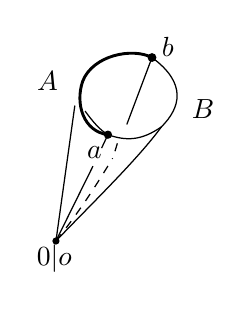
\begin{tikzpicture}[x=1cm,y=1cm,line width=.45pt]
\coordinate (o) at (0,0);
\coordinate (a) at (.66,1.35);
\coordinate (b) at (1.22,2.33);
\draw[line width=1.05pt] (a)
  .. controls (.35,1.39) and (.24,1.74) .. (.34,2.03)
  .. controls (.47,2.36) and (.97,2.46) .. (b);
\draw (.37,1.65) .. controls (.48,1.50) and (.56,1.41) .. (a);
\draw (b)
  .. controls (1.67,2.00) and (1.58,1.69) .. (1.34,1.45)
  .. controls (1.08,1.27) and (.89,1.27) .. (a);
\draw (o) -- (.24,1.72);
\draw (o) .. controls (.48,.50) and (1.04,1.04) .. (1.34,1.45);
\draw (b) -- (.90,1.48);
\draw[dashed] (o) .. controls (.36,.45) and (.59,.84) .. (.72,1.05);
\draw (.75,1.14) -- (.78,1.24);
\draw (o) -- (.47,.95);
\draw (a) -- (.58,1.18);
\fill (a) circle (1.5pt);
\fill (b) circle (1.6pt);
\fill (o) circle (1.3pt);
\node[left] at (.15,2.03) {$A$};
\node[right] at (1.60,1.67) {$B$};
\node at (.49,1.12) {$a$};
\node at (1.42,2.47) {$b$};
\node at (-.02,-.22) {$\unsure{0|o}$};
\end{tikzpicture}}}

Pour tout $x\in X$, considérons \inserted{l'ens $I_x\subset I$} des $i\in I$ tels
que $X_i\ni x$ --- il y en a un nb fini, \deleted{et}
(par (1' \unsure{a|0})), et l'ens de ces $I$ est filtrant
décroissant par (21 d), donc il y a
un plus petit $i\in I_x$ \deleted{tel que}, soit $i(x)$
\[
(25)\qquad i(x)=\text{plus petit des }i\in I\text{ tels que }x\in X_i.
\]
Soit d'autre part, pour tout $i\in I$
\margin{53}

\scanpage{55}
\mspage{15}
\[
(26)\qquad
\underset{\text{fermé de }X_i}{\dot X_i\overset{\text{déf}}=\bigcup_{j<i}X_j},
\qquad
\underset{\text{ouvert de }X_i}{X_i^*\overset{\mathrm{def}}=X_i\setminus\dot X_i}.
\]

\margin{\uline{NB} On n'exclut pas que certains des $X_i$ soient $=\phi$ $\bar m$ si $X_i\ne\phi$. Sauf erreur, ``il n'y a pas d'inconvénient'' à remplacer $I$ par le \unsure{sous. ens|sous-ens. ord.} de $I$ formé des $i$ tels que $X_i^*\ne\phi$ \unsure{clairem\textsuperscript{t}|clairement} $(X_i)_{i\in I'}$ \deleted{\unsure{sa|ca}} \deleted{\unsure{d'ailleurs}} \inserted{\unsure{satisfont}} \deleted{\unsure{satisfont}} aux $=$ conditions a) b) c) d)}

\uline{Proposition} Les $X_i^*$ sont mutuellement disjoints, et leur réunion est $X$. Si $x\in X$, $i(x)$ est aussi l'unique $i\in I$ tel que $x\in X_i^*$.

\uline{Dém.} Soit $x\in X_i^*\cap X_j^*$ ($i,j\in I$, $i\ne j$), donc \deleted{\unsure{alors}} $x\in X_i\cap X_j$ \deleted{(\unsure{car})}, donc $\exists k\leq i,j$ avec
\deleted{$\unsure{x\in X_i\cap X_j=}$}
$x\in X_k$ si on avait $k=i$ on aurait $i\leq j$ donc $i<j$ absurde car $x\in X_j^*\subset X_j\setminus X_i^*$.
Or $k<i$ donc $x\in X_i\setminus X_k$ ce qui contredit $x\in X_i^*$. Donc les $X_i^*$ mutuellement \unsure{disjoint|disjoints}. D'ailleurs $x\in X_{i(x)}^*$ est trivial par définition de $i(x)$, d'où la prop.

On posera
\[
(27)\qquad
\left\{\begin{aligned}
\dot X_{\Delta_0}&=\coprod_{i\in I}\dot X_i\\
X_{\Delta_0}^*&=\unsure{:}X_{\Delta_0}\setminus\dot X_{\Delta_0}=\coprod_{i\in I}X_i^*,
\end{aligned}\right.
\]
puis \deleted{\unsure{par}} plus généralement
\[
(28)\qquad
\begin{aligned}
&\left\{\begin{aligned}
\dot X_{\Delta_r}&=\text{image inverse de }\dot X_{\Delta_0}\text{ par}\\
&\qquad\sigma_r:X_{\Delta_r}\longrightarrow X_{\Delta_0}
\qquad\text{\uline{fermé} de }X_{\unsure{\Delta_r|\Delta_0}}\\
\underset{\text{ouvert de }X_{\Delta_r}}{X_{\Delta_r}^*}&=X_{\Delta_r}\setminus\dot X_{\Delta_r}=\text{image inv. de }X_{X_0}^*
\end{aligned}\right.\\
&\qquad\text{par }\sigma_r:X_{\Delta_r}\longrightarrow X_{\Delta_0}.
\end{aligned}
\]
\margin{54}

\scanpage{56}
Si
\[
\alpha:\Delta_{r'}\longrightarrow\Delta_r,\qquad \text{\uuline{$\alpha(\unsure{0|\omega})=0$}},
\]
\[
(29)\qquad\left\{\begin{aligned}
&\text{alors}\qquad \alpha^*:X_{\Delta_r}\mathbin{\unsure{-|\longrightarrow}}X_{\Delta_{r'}}\qquad(\text{étale})\\
&\text{satisfait}\\
&\qquad\alpha^*(X_{\Delta_{r'}}^*)=X_{\Delta_r}^*,\quad\text{ie. }\alpha^*(\dot X_{\Delta_{r'}})=\dot X_{\Delta_r}.
\end{aligned}\right.
\]

\deleted{\unsure{Dans le cas}}

\uline{NB} ``Moralement'', $X_{\Delta_r}^*$ représente une sorte de partie ``non \unsure{singulière|singulier}'' de $X_{\Delta_r}$, $\dot X_{\Delta_r}$ la partie singulière ou ``bord''. On fera attention que les $X_{\Delta_r}^*$ ne \uline{forment} \uline{pas} un espace semi-simplicial.

Pourtant, notre propos est, dans une certaine mesure, de reconstituer $X$ à partir des ``strates ouvertes'' $X_i^*$ dans $X$, dans l'esprit du n° 1 (où il y a deux strates $X_0=Y$ et $X_1=X$, \deleted{$\unsure{Y\subset X}$ \unsure{fermé}} \inserted{($Y\subset X$ inclusion} fermée), et on a donc $Y=Y^*$, $X^*=X\setminus Y$ comme dans les notations du loc. cit, où il y avait lieu d'introduire $\mathcal{V}_{\unsure{Y},X}$.
\margin{55}

\scanpage{57}
\mspage{16}
3. \uline{Stratifications globales} : \uline{introduction \unsure{aux} tubes}

On garde les notations précédentes.

Pour tt couple $(i\leq j)\in I\times I$, considérons
\[
(1)\qquad \overline{\mathcal V}_{i,j}=\mathcal V^{\ell}_{X_i,X_j}\qquad
\begin{gathered}\text{voisinage tubulaire}\\\text{de }X_i\text{ dans }X_j\end{gathered}
\]
(cf § 1\unsure{)}, et posons
\[
(2)\qquad\dot{\mathcal V}_{i,j}=\deleted{\unsure{\mathcal V_{ij}|\overline{\mathcal V}_{ij}}}\ \overline{\mathcal V}_{ij}\cap\bigl(\deleted{\unsure{R_j}}\inserted{\unsure{R|a}_{i,j}^{\deleted{\unsure{*}}}}\bigr)=\overline{\mathcal V}_{ij}\cap R_i
\]

où on pose, pour $i,j\in I$
\[
(3)\qquad R_{i,j}^{\deleted{\unsure{*}}}=\left(
\underbrace{\bigcup_{\substack{k\in I\ \text{tels que}\\\deleted{\unsure{X_k}}\ X_k\not\supset X_i}}X_k}_{\substack{R_i\ \text{partie fermée}\\\text{de }X}}
\right)\cap X_j
\]
\deleted{$(\unsure{\bigcup}_{k<j\ \unsure{\text{tel q}}}$}

\margin{\uline{NB} On a aussi
\[
(3\mathrm{bis})\qquad R_{ij}=\bigcup_{\substack{\underline{k<}j\\\text{tel que }X_k\cap X_i\ne X_i}}X_k\subset\dot X_j
\]}

On notera qu'on a
\[
(4)\qquad R_{i\deleted{j}}\cap X_i=R_{ij}\cap X_i=\dot X_i.
\]

En effet, si $X_k\not\supset X_i$ i.e. $X_k\cap X_i\subsetneq X_i$, comme $X_k\cap X_i=\bigcup_{\ell\leq k,i}X_\ell$, on voit que \deleted{$X_k\cap X_i\ \unsure{\text{et}}\ \ell<i$} $\ell\leq k,i$ implique $X_\ell\subsetneq X_i$ d'où $\ell<i$ et $X_\ell\subset\dot X_i$, donc $X_k\cap X_i\subset\dot X$, d'où $R_i\cap X_i\subset\dot X_i$ — l'inclusion en sens inverse étant triviale.
\margin{56}

\scanpage{58}
On posera \deleted{enfin}
\[
(5)\qquad \mathcal{V}_{ij}=\overline{\mathcal{V}}_{ij}\setminus\dot{\mathcal{V}}_{ij}=\overline{\mathcal{V}}_{ij}-\overline{\mathcal{V}}_{ij}\cap R_{ij}
\]
qui est donc un espace infinitésimal autour de
\[
(6)\qquad \mathcal{V}_{ij}\cap X_i=X_i^*.
\]
Je poserai enfin
\[
(7)\qquad\begin{aligned}
\mathcal{V}_{ij}^*&=\overline{\mathcal{V}}_{ij}\setminus\bigcup_{\deleted{\unsure{i|\ell}}\,\text{\uline{$k$}}<j}X_k\cap\overline{\mathcal{V}}_{ij}\\
&=\overset{\deleted{\unsure{-}}}{\overline{\mathcal{V}}}_{ij}\setminus\dot X_j\\
&=\mathcal{V}_{ij}\cap X_j^*\subset\mathcal{V}_{i,j}.
\end{aligned}
\]
Notons que pour $i=j$, on trouve
\[
(8)\qquad\overline{\mathcal{V}}_{ii}=X_i,\quad\dot{\mathcal{V}}_{i,i}=\dot X_i,\quad\text{\uline{$\mathcal{V}_{i,i}=\mathcal{V}_{i,i}^*=X_i^*$}}
\]
Nos ``pierres'' de construction, dans une première étape, vont être les $\mathcal{V}_{i,j}^*$, $\mathcal{V}_{ij}$ avec les inclusions évidentes
\diagram{(9)\qquad\begin{tikzcd}[column sep=large,row sep=small]
& X_i^*\arrow[d,"\text{``âme''}"]\\
\unsure{\mathcal{V}_{ij}^*|X_{ij}^*}\arrow[r]\arrow[d] & \mathcal{V}_{i,j}\\
X_j^* &
\end{tikzcd}}
,
ces pierres \unsure{comprenant|comprennent} \inserted{les} $X_i^*$ comme
\margin{57}

\scanpage{59}
\mspage{17}
cas particulier, en faisant $i=j$.

À vrai dire, je vois maintenant que ces fameuses pierres telles quelles sont des côtes mal taillées — ils sont trop \unsure{généraux|généreux}, ou pas assez. Pas assez pour contenir les morceaux $\unsure{\mathcal V|\dot{\mathcal V}}_{d_*,d''_*}^{d'_*}\approxeq\unsure{\check N|\widetilde N}_{d_*;(d'_0,d''_0)}\mid D_{d_*}^*$ de ($\mathrm{Str}_\infty$ p. 84) — trop en ce sens, que l'on peut s'en tirer avec des ``pierres'' plus petites pour ainsi dire certaines des précédentes, correspondant au cas où $j$ est un \uline{successeur} de $i$ (i.e. $\nexists h$ avec $i<h<j$).
Ces pierres sont \inserted{particulièrement} intéressantes, en ce sens que pour des hypothèses de lissité et de locale trivialité normale (ou ``équisingularité'') convenables du type \unsure{standart|Standart} (et sûrement réalisables p. ex. pour tt variété alg. complexe, munie de sous-variétés alg. complexes fermées)) $\mathcal V_{i,j}^*$ \deleted{\unsure{est}} homéomorphe$ {}^*$ \unsure{à|:} un fibré sur $X_i^*$ \unsure{(}qui est une variété topologique) \unsure{à|:} fibre une variété topologique, et $\bar m$ à fibre un cylindre ouvert : $\mathbb R\times C_{i,j}$ \inserted{($\simeq Z_{ij}^*=Z_{i,j}\setminus\{z\}$)} (où $\unsure{C_{ij}|C_j}$ est une \uline{variété top compacte} (NB $\mathcal V_{i,j}$ serait homéomorphe \unsure{à|:} un fibré en \uline{cônes} sur $C_{ij}$ \ldots). Quand $j$ n'est pas un successeur de $i$, alors $C_{ij}$ sera encore une variété, mais non compacte. Quand

\margin{\uline{\uuline{NB}} Mais ce dessin (dans le domaine réel) dessine une situation pas tellement vraisemblable — qui ne correspond pas vraiment aux ``hyp. \ldots\ convenables de type \unsure{standart|Standart}'' la str.te
\figure{\begin{tikzpicture}[x=1cm,y=1cm]
\draw (0,0)--(3,0);
\fill (1.42,0) circle (1.8pt);
\node[above] at (.25,0) {$X_i$};
\end{tikzpicture}}
devrait se décomposer en tous cas en deux.}

\margin{$ {}^*$ du moins si $X_i^*=X_i$\unsure{,} i.e $\dot X_i=\phi$, sinon on peut avoir \deleted{\unsure{des cas}} des situations comme dans le dessin
\figure{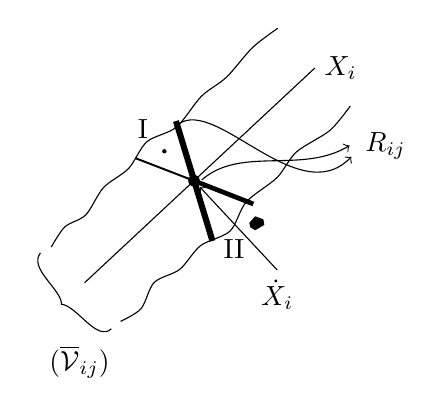
\begin{tikzpicture}[x=1cm,y=1cm,rotate=43]
\draw (0,0)--(4,0) node[right] {$X_i$};
\draw plot[smooth] coordinates {(0,.62)(.3,.69)(.6,.62)(1,.72)(1.4,.68)(1.8,.77)(2.2,.65)(2.7,.72)(3.1,.68)(3.6,.73)(4,.69)};
\draw plot[smooth] coordinates {(0,-.67)(.3,-.73)(.65,-.6)(1,-.7)(1.4,-.66)(1.8,-.78)(2.2,-.65)(2.7,-.69)(3.1,-.62)(3.6,-.71)(4,-.66)};
\draw[line width=.7pt] (1.55,.72)--(1.9,0);
\draw[line width=1.7pt] (1.9,0)--(2.25,-.73);
\draw[line width=2.2pt] (1.55,-.72)--(2.25,.71);
\fill (1.9,0) circle (2.1pt);
\fill (1.88,.53) circle (.8pt);
\fill (2.05,-.87)--(2.16,-.86)--(2.21,-.96)--(2.17,-1.02)--(2.04,-.99)--(2.02,-.92)--cycle;
\node at (1.87,.92) {$\mathrm I$};
\node at (1.68,-.98) {$\mathrm{II}$};
\draw[->] (1.9,-1.55)--(1.9,-.11);
\node[below] at (1.9,-1.55) {$\dot X_i$};
\draw[->] (2.18,.66) .. controls (2.85,.72) and (2.58,-1.20) .. (3.57,-1.14);
\draw[->] (1.98,-.06) .. controls (2.64,-.08) and (2.96,-.88) .. (3.65,-1.02);
\node[right] at (3.7,-1.08) {$R_{ij}$};
\draw (-.15,-.66) .. controls (-.4,-.66) and (-.27,-.15) .. (-.4,0) .. controls (-.27,.14) and (-.4,.62) .. (-.15,.66);
\node[below left] at (-.14,-.8) {$(\unsure{\overline{\mathcal V}_{ij}})$};
\end{tikzpicture}}
où dans $\mathcal V_{ij}^*$ il y a des morceaux suppl. ``idiots'' I et II \ldots}
\margin{58}

\scanpage{60}
aux espaces (plutôt, germes d'espaces --- \unsure{topos|topo}) \deleted{$\unsure{\mathcal V_{ij}}$} plus généraux que les $\mathcal V_{ij}^*$ (et les $\mathcal V_{ij}$), ce sont les suivants : on considère
\[
i\leq j\leq k\qquad\text{d'où}\qquad X_i\subset X_j\subset X_k
\]
on prend
\[
(10)\qquad \mathcal V_{i,k}^j\overset{\text{déf}}=\overline{\mathcal V}_{X_i,X_k}\setminus(R_{\deleted{\unsure{j}}\inserted{i},k}\cup\unsure{S_{j,k}|\Sigma_{j,k}})\ \unsure{\deleted{m}|\underline{m}}
\]
où $R_{i,k}$ est défini dans (3) (3bis), et où
\[
(11)\qquad S_{j,k}\overset{\text{déf}}=\bigcup_{\substack{\ell\in I\\\text{avec}\\j\leq\ell<k}}X_\ell
\]
\margin{(\uline{NB} $S_{j,k}=\phi$ si $j=k$\\
$S_{j,k}=X_j$ si $k$ \unsure{succ.|success.}\\
de $j$)}

(On a, en comparant avec (3bis), une \inserted{ps-}partition de l'ens $I^{(k)}\overset{\deleted{\unsure{\mathrm{def}|\text{déf}}}}=\{\ell\in I\mid\unsure{\ell<k|\ell\leq k}\}$ en deux parties,
\[
I^{*(k)'}=\{\ell\in I^{(k)}\mid X_\ell\unsure{\not\supset|\not\supseteq}X_j\}\quad\text{et}\quad
I^{(k)''}=\{\ell\in I^{(k)}\mid X_\ell\supset X_j\},
\]
et on a
\[
(12)\qquad\left\{\begin{aligned}
R_{j,k}&=\bigcup_{\ell\in I^{(k)'}}X_\ell\\
S_{j,k}&=\bigcup_{\ell\in\unsure{I^{(k)''}|I^{(k)'}}}X_\ell,
\end{aligned}\right.
\qquad\begin{gathered}
\text{Donc }R_{j,k}\cup S_{j,k}=\dot X_k\\
(\text{aussi }R_{j,\unsure{k|n}}\cap S_{j,k}=\dot X_i)
\end{gathered}
\]
\deleted{$\unsure{\mathcal V_{ij}}$} On a donc
\[
(13)\qquad \mathcal V_{i,k}^i=\mathcal V_{i,k}^*,\qquad \mathcal V_{i,k}^k=\mathcal V_{i,k},\qquad
\begin{gathered}
\text{\inserted{d'où}}\ \mathcal V_{i,i}^i=\mathcal V_{i,i}=\mathcal V_{i,i}^*\\[-2pt]
\hspace{2.6cm}\makebox[0pt][l]{\begin{tikzpicture}[baseline=0pt]
\path[use as bounding box] (0,-.5) rectangle (0,.8);
\draw[overlay,line width=.45pt] (-.08,.03) .. controls (-.09,.39) and (.08,.43) .. (.26,.43)
  -- (1.35,.70) -- (1.36,-.40) .. controls (1.33,-.47) and (1.20,-.48) .. (1.09,-.49);
\draw[overlay,line width=.4pt] (1.28,.62) -- (1.40,.78);
\end{tikzpicture}}=X_i^*
\end{gathered}
\]

$\mathcal V_{i,k}^j$ a encore tendance à être \deleted{\unsure{un}} homéomorphe (ou du moins, homotope, ou homéomorphe en un sens affaibli de germes, \unsure{o} qu'il faudrait dégager\ldots) à un fibré loc. trivial de base $X_i^*$, mais comme on voit déjà dans le cas $\mathcal V_{i,k}^k=\mathcal V_{i,k}$) à fibre pouvant être singulière. Dans le cas de $\mathcal V_{i,k}^k$,
\margin{59}

\scanpage{61}
% His upper-right number; only the lower, open oval frame survives at the clipped top edge.
\mspage{\makebox[0pt][l]{\begin{tikzpicture}[overlay,baseline=0pt]
\draw (-.22,.15) .. controls (-.24,-.22) and (.55,-.22) .. (.54,.15);
\end{tikzpicture}}18}
avec $k$ successeur de $i$, il s'agit de singularité isolée, mais dans le cas de $\mathcal{V}_{i,k}^k$ général, on peut trouver des singularités de type arbitraire bien sûr en fibre (prendre $X_i=X_i^*$ réduit à un pt !) — ce qui diminue l'intérêt, dans le cas de stratifications tant soit peu générales, des $\mathcal{V}_{i,k}^j$ généraux comme ``pierres''. Les $\mathcal{V}_{i,k}^{j}=\mathcal{V}_{i,k}^*$ sont déjà plus intéressants, car \deleted{\unsure{ce sont}} c'est essentiellement un \inserted{germe d'} ouvert de $X_k^*$, donc non singulier — ce qui \unsure{s'exprimera|s'exprime} par le fait qu'on l'obtient comme un fibré sur $X_i^*$ non singulier, à fibre non singulière $\mathcal{V}_{\unsure{z|Z},Z_{i,k}}^*$ \ldots

Donc nous allons dans la suite systématiquement essayer d'exprimer le maximum avec les $X_i^*$ et \inserted{les} $\mathcal{V}_{i,j}$, $\mathcal{V}_{i,j}^*$ ``élémentaires'' ($j$ successeur de $i$), puis voir si certaines expressions peuvent prendre une forme plus sympathique en utilisant aussi \inserted{les $X_i^*$ et} les $\mathcal{V}_{\unsure{i,j|ijj}}$, $\mathcal{V}_{i,j}^*$ avec $i\leq j$ \unsure{sans|dans} plus — et dans un dernier temps seulement, peut-être (\unsure{en|eu} égard au cas des diviseurs \unsure{à|:} croisements normaux) voir comment les $\mathcal{V}_{i,k}^j$ s'insèrent dans ce formalisme.
% Pale lower-left foliation, another hand.
\margin{60}
